\subsection{Case studies}
\label{subsec:noah__case_studies}

Using all that has been described in the previous sections, we now look at a few `typical' supersequences to understand their construction.
A quick note about the nomenclature of NOAH supersequences is warranted here.
Supersequences are labelled by the number of modules $N$, plus a series of single-letter codes corresponding to the identity and ordering of the modules involved (\cref{tbl:noah_modules}).
Occasionally, superscripts or subscripts are used to qualify the modules involved.%
\footnote{With the increasing number of modules, and the variety of modern NMR experiments which could be incorporated into NOAH supersequences, keeping these abbreviations short yet meaningful has been a challenge.}
Thus, a NOAH supersequence containing three modules---say \nitrogen{} HMQC, \carbon{} HSQC, and CLIP-COSY---would be referred to as a \noah{Mn,S,Cc}.
\Cref{tbl:noah_sensitivities} provides values of $\rho_t$ and $A$ for each module of several typical supersequences, which will be rationalised in the text which follows.

\begin{table}[!ht]
    \begin{tabular}{cccccc}
        \toprule
        \multicolumn{2}{c}{\textbf{\proton{}--\nitrogen{} modules}}  &
        \multicolumn{2}{c}{\textbf{\proton{}--\carbon{} modules}}    &
        \multicolumn{2}{c}{\textbf{\proton{}--\proton{} modules}}   \\
        \cmidrule(lr){1-2}
        \cmidrule(lr){3-4}
        \cmidrule(lr){5-6}
        Module & Code        & Module     & Code           & Module     & Code       \\
        \midrule
        HMQC   & \noah*{Mn}  & HSQC       & \noah*{S}      & COSY       & \noah*{C}  \\
        HSQC   & \noah*{Sn}  & seHSQC     & \noah*{Sp}     & CLIP-COSY  & \noah*{Cc} \\
        seHSQC & \noah*{Spn} & HSQC-TOCSY & \noah*{St}     & DQF-COSY   & \noah*{D}  \\
        HMBC   & \noah*{Bn}  & HSQC-COSY  & \noah*{Sc}     & TOCSY      & \noah*{T}  \\
               &             & 2BOB       & \noah*{O}      & NOESY      & \noah*{N}  \\
               &             & HMBC       & \noah*{B}      & ROESY      & \noah*{R}  \\
               &             & ADEQUATE   & \noah*{A}      & PSYCHE     & \noah*{P}  \\
               &             &            & \hspace{1.5cm} & TSE-PSYCHE & \noah*{Pt} \\
               &             &            &                & PSYCHE 2DJ & \noah*{J}  \\
        \bottomrule
    \end{tabular}
    % The hspace is to make the two subcolumns look more balanced.
    \caption[List of single-letter NOAH module codes]{
        A (non-exhaustive) list of single-letter module codes for a selection of NOAH modules.
        Note that, in the literature, the \nitrogen{} HMQC module has been referred to simply by `M', since the HSQC module is preferred for \proton{}--\carbon{} correlations.
        In this thesis, I include the subscript N throughout to avoid any ambiguity.
    }
    \label{tbl:noah_modules}
\end{table}

\begin{table}[!ht]
    % data is in lab book: noah-misc/220224/
    \begin{tabular}{ccccccccc}
        \toprule
        \textbf{Entry} & \textbf{Sequence} & $\symbf{\tau}_{\textbf{NOAH}}$ & $\symbf{\rho}_{\symbfit{t}}$ & \multicolumn{5}{c}{$\symbfit{A}$} \\
        \cmidrule(lr){5-9}
        & & & & HMBC & seHSQC & HSQC & COSY & TOCSY \\
        \midrule
        1 & \noah*{S,C}         & 15 min 0 s  & 1.87 &      &      & 0.97 & 0.90 &      \\
        2 & \noah*{S,C,T}       & 16 min 25 s & 2.60 &      &      & 1.01 & 0.99 & 0.79 \\
        3 & \noah*{B,S}         & 15 min 40 s & 1.82 & 0.93 &      & 0.87 &      &      \\
        4 & \noah*{S,B}         & 15 min 35 s & 1.83 & 0.99 &      & 0.96 &      &      \\
        5 & \noah*{B,S,C,T}     & 17 min 48 s & 3.22 & 0.95 &      & 0.90 & 0.36 & 0.28 \\
        6 & \noah*{B,Spn,S,C,T} & 18 min 57 s & 3.74 & 0.95 & 0.71 & 0.66 & 0.38 & 0.30 \\
        7 & \noah*{Spn,B,S,C,T} & 18 min 56 s & 3.75 & 0.76 & 0.79 & 0.74 & 0.33 & 0.26 \\
        \bottomrule
    \end{tabular}
    \caption[Sensitivity and time-saving analyses of several NOAH supersequences]{
        Sensitivity and time-saving analyses of several typical NOAH supersequences.
        All experiments were acquired with 2 scans per increment, 256 $t_1$ increments, an acquisition time of \qty{67}{\ms}, and a recovery delay of \qty{1.5}{\s}.
        The HMBC module used here includes the extra \carbon{} \ang{90} pulse described later in \cref{subsec:noah__hmbc}: this has no significant impact on the SNR, and is only mentioned as a technicality.
        The \nitrogen{} seHSQC module is that described in \cref{subsec:noah__sehsqc_n}.
        The CT module here was run with States indirect-dimension quadrature detection, and the individual C module (in entry 1) with echo--antiecho.
        The following Bruker library sequences were used as the `conventional' experiments: \texttt{hmbcetgpl2nd}, \texttt{hsqcetf3gpsi2}, \texttt{hsqcetgpsp.2}, \texttt{cosygpqf}, and \texttt{dipsi2gpphzs}.
        \datacode{7Z-220224}
    }
    \label{tbl:noah_sensitivities}
\end{table}

\subsubsection{\noah{S,C}: HSQC + COSY}

We begin with perhaps the simplest example of a NOAH supersequence, one containing the HSQC and COSY modules: this is labelled as a \noah{S,C} experiment (entry 1, \cref{tbl:noah_sensitivities}).
As shown in \cref{fig:noah_sb_po_s}, the HSQC module only samples \magn{C} magnetisation, and leaves \magnnot{C} magnetisation along the $+z$-axis
Although the HSQC experiment has to be modified to preserve this \magnnot{C} magnetisation, its sensitivity is practically unaffected as compared to a `standard' HSQC ($A = 0.97$).
Furthermore, the COSY module retains \textit{most} of its sensitivity ($A = 0.90$).
The small loss here is because the HSQC module does not \textit{perfectly} preserve the \magnnot{C} magnetisation: for example, evolution of J-couplings as well as relaxation occur during the HSQC pulse sequence, which are ignored in the product operator analysis in \cref{fig:noah_sb_po_s}.

The value of the time-saving factor, $\rho_t = 1.87$, is very close to the theoretical limit of $N = 2$.
This reflects the fact that the pulse sequence itself, $\tau_\text{ps}$, is fairly short for both the HSQC and COSY modules; the deviation therefore chiefly arises from the acquisition time, $\tau_\text{acq}$.
In all respects, this is therefore an example of an `ideal' NOAH supersequence, where the combination of two modules provides time savings without compromising on sensitivity.

It is worth pointing out that the order of the modules cannot be reversed: the COSY module cannot be (easily) modified to preserve \magn{C} magnetisation.
In a hypothetical \noah{C,S} supersequence, the later HSQC module would only be able to use magnetisation recovered during the COSY FID, leading to substantial sensitivity drops.

\begin{figure}[!ht]
    \centering
    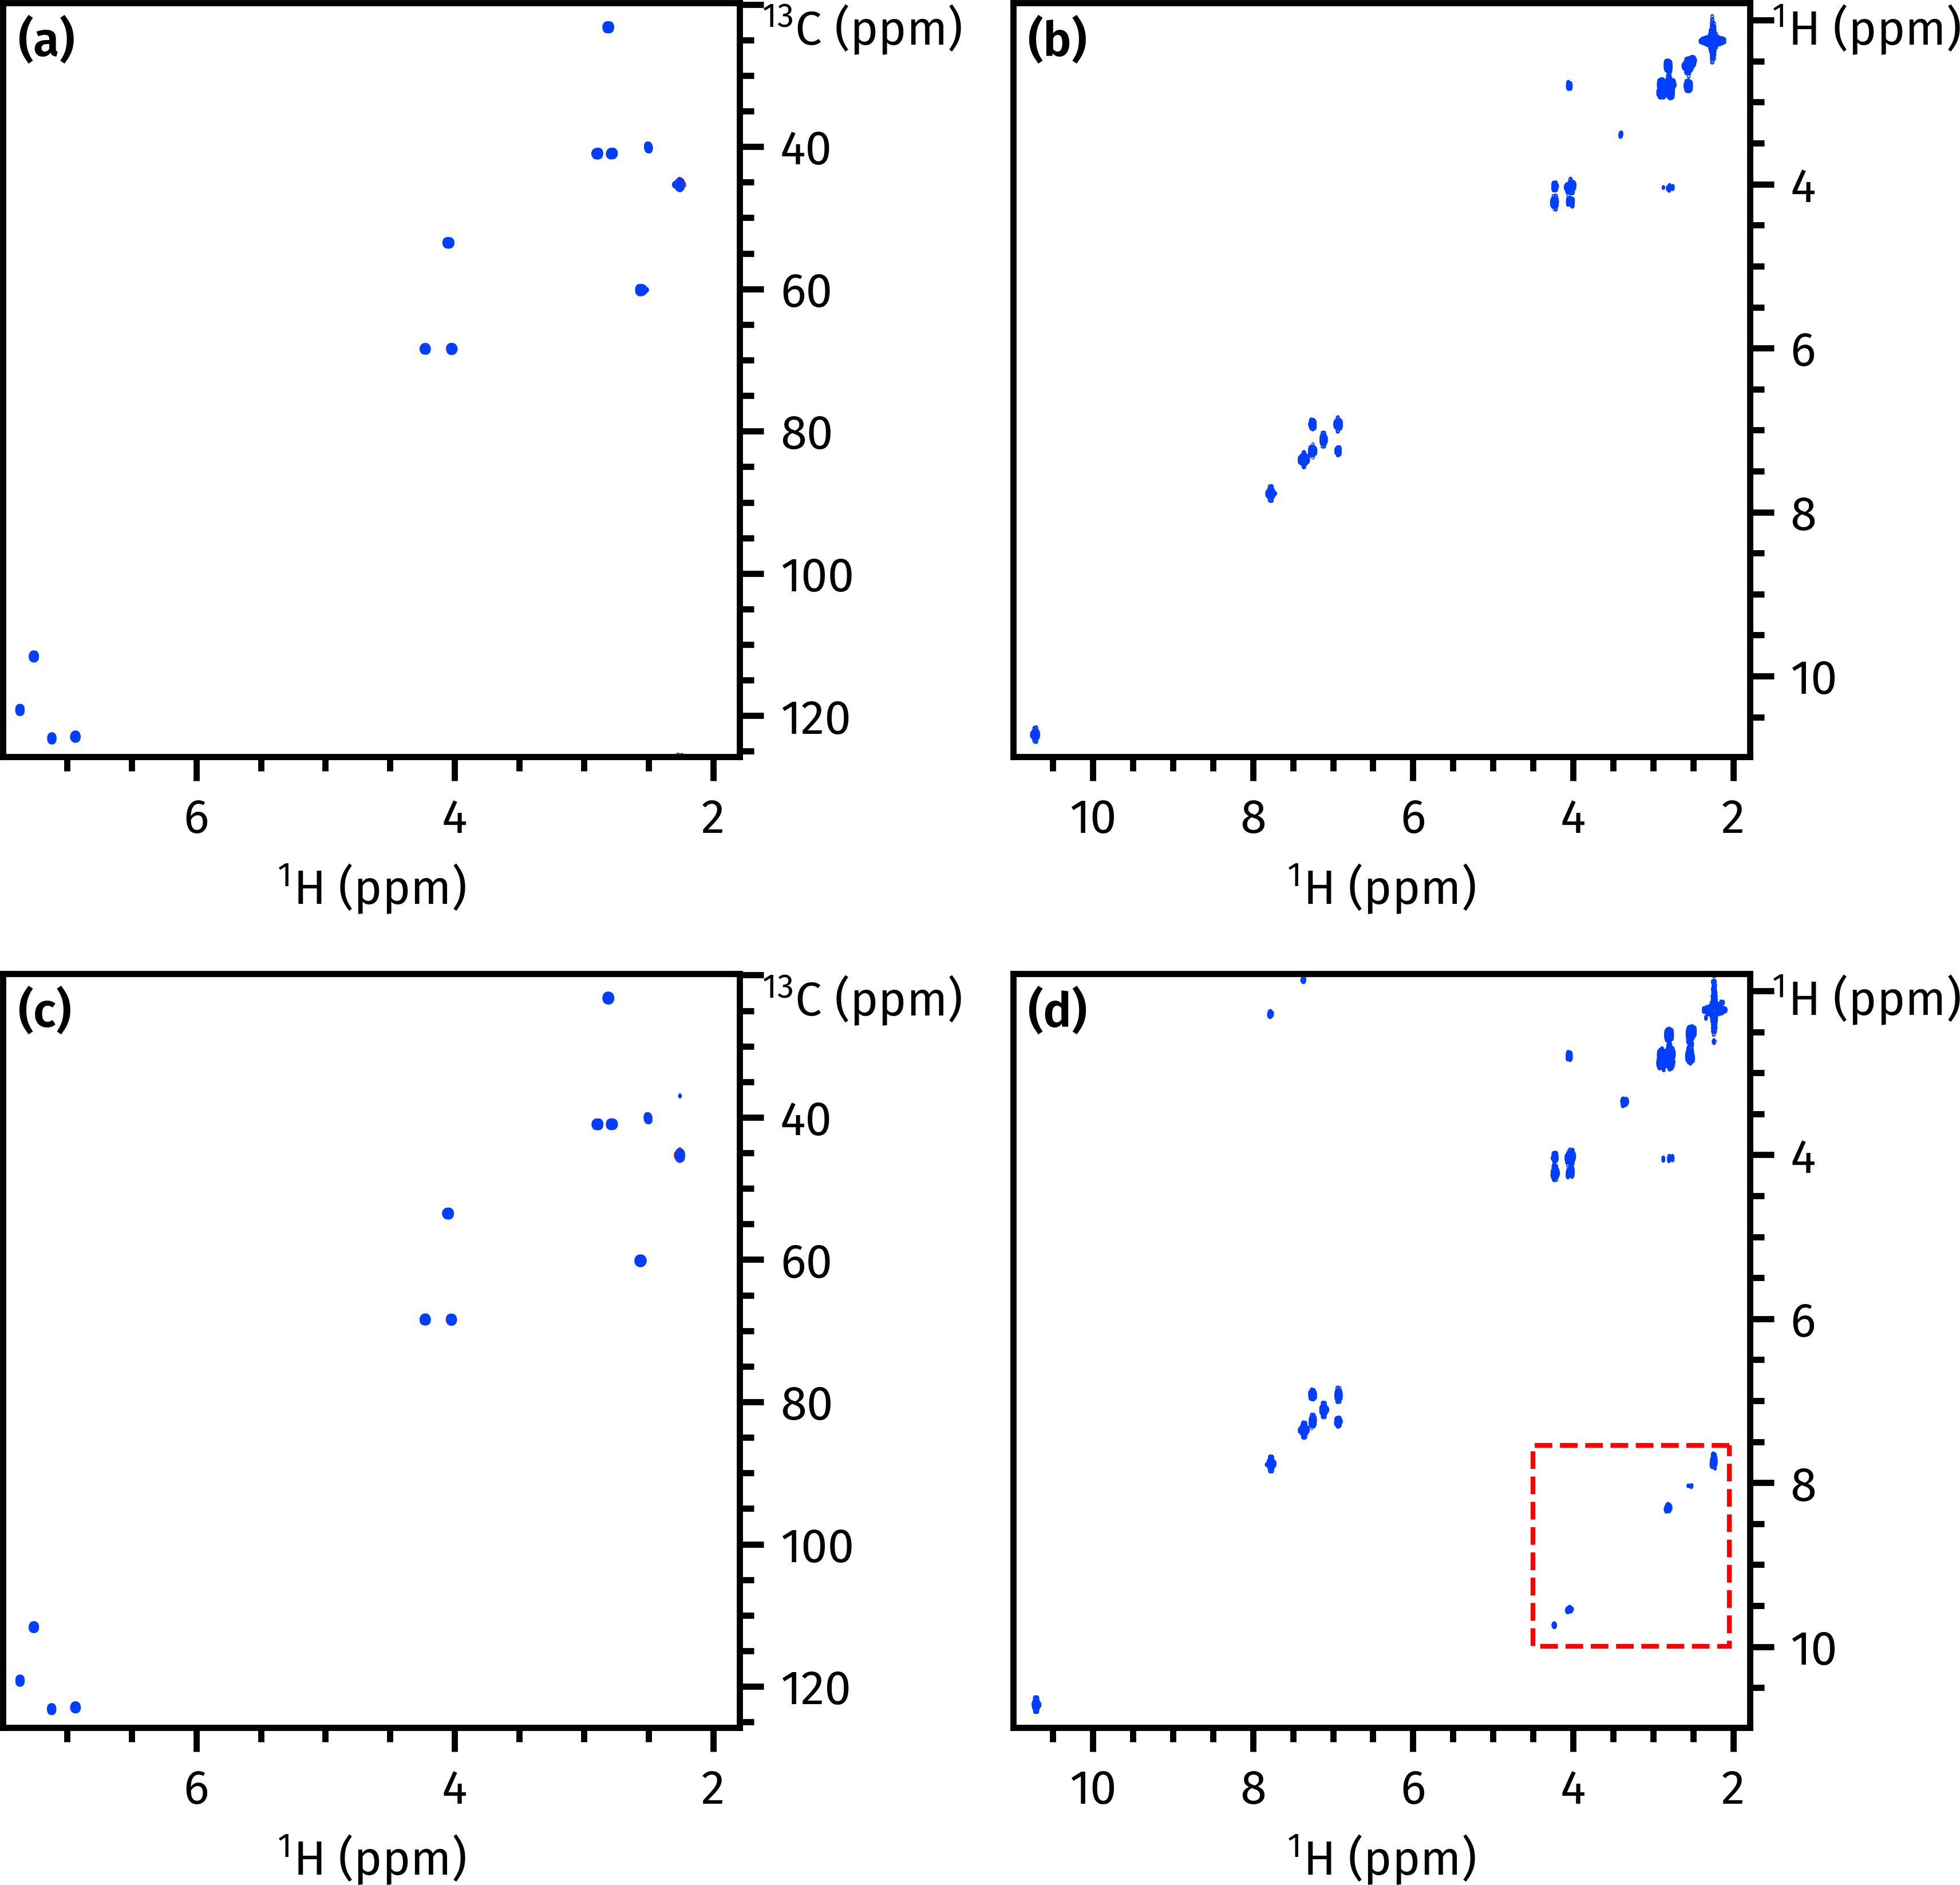
\includegraphics[]{noah/sc_noah_vs_conv.png}%
    {\phantomsubcaption\label{fig:sc_noah_vs_conv_noah_s}}%
    {\phantomsubcaption\label{fig:sc_noah_vs_conv_noah_c}}%
    {\phantomsubcaption\label{fig:sc_noah_vs_conv_conv_s}}%
    {\phantomsubcaption\label{fig:sc_noah_vs_conv_conv_c}}%
    \caption[Comparison of spectra obtained from \noah{S,C} and standalone experiments]{
        \textbf{(\subref{fig:sc_noah_vs_conv_noah_s})} HSQC from \noah{S,C} supersequence.
        \textbf{(\subref{fig:sc_noah_vs_conv_noah_c})} COSY from \noah{S,C} supersequence.
        \textbf{(\subref{fig:sc_noah_vs_conv_conv_s})} Standalone HSQC.
        \textbf{(\subref{fig:sc_noah_vs_conv_conv_c})} Standalone COSY; off-diagonal artefacts are highlighted in the red box.
        \datacode{7Z-220224}
    }
    \label{fig:sc_noah_vs_conv}
\end{figure}

A final point to consider would be whether the NOAH data has comparable spectral quality in terms of (for example) artefacts.
In this case, the answer is yes: the NOAH HSQC spectrum is virtually identical to the standalone (\cref{fig:sc_noah_vs_conv_noah_s,fig:sc_noah_vs_conv_conv_s}; both spectra have low-level artefacts of different kinds, which do not seriously impede the interpretation and are not shown).
On the other hand, the NOAH COSY spectrum seems to actually \textit{improve} on the standalone COSY, in that it better suppresses off-diagonal artefacts (\cref{fig:sc_noah_vs_conv_noah_c,fig:sc_noah_vs_conv_conv_c}).
These artefacts likely arise in the standalone COSY because of accidental refocusing of magnetisation which has not completely relaxed between $t_1$ increments.\autocite{Vitorge2010JMR}
In contrast, the NOAH COSY module has an extra set of HSQC gradients between every repetition of the COSY, so accidental refocusing is less likely.
(Similar artefacts have been noted before in the DQF-COSY experiment\autocite{Shaw1996JMRSA,Howe2014MRC}, and have also shown to be attenuated in the corresponding NOAH module\autocite{Claridge2019MRC}.)
That said, such improvements are not always guaranteed: there are sometimes artefacts which arise uniquely in NOAH experiments, some of which are discussed in the following sections.


\subsubsection{\noah{S,C,T}: HSQC + COSY + TOCSY}

Evidently, the fact that the HSQC preserves almost all \magnnot{C} magnetisation means that \textit{any} homonuclear module---or a combination thereof---can be placed after it.
In general, since homonuclear modules tend to consume any remaining bulk magnetisation, it is very difficult to create combinations of homonuclear modules which do not lead to significant reductions in sensitivity.
The only real exceptions are COSY/X combinations, where X can be NOESY, ROESY, or TOCSY: instead of concatenating the COSY and X modules, the COSY pulse sequence can instead be nested \textit{within} the X module, as was first demonstrated with X = NOESY\autocite{Haasnoot1984JMR,Gurevich1984JMR}.
Here, we use the COSY/TOCSY combination as an example.\autocite{Nolis2019MRC}
The COSY, TOCSY, and combined COSY/TOCSY modules are shown in \cref{fig:ct_states}.

\begin{figure}[!ht]
    \centering
    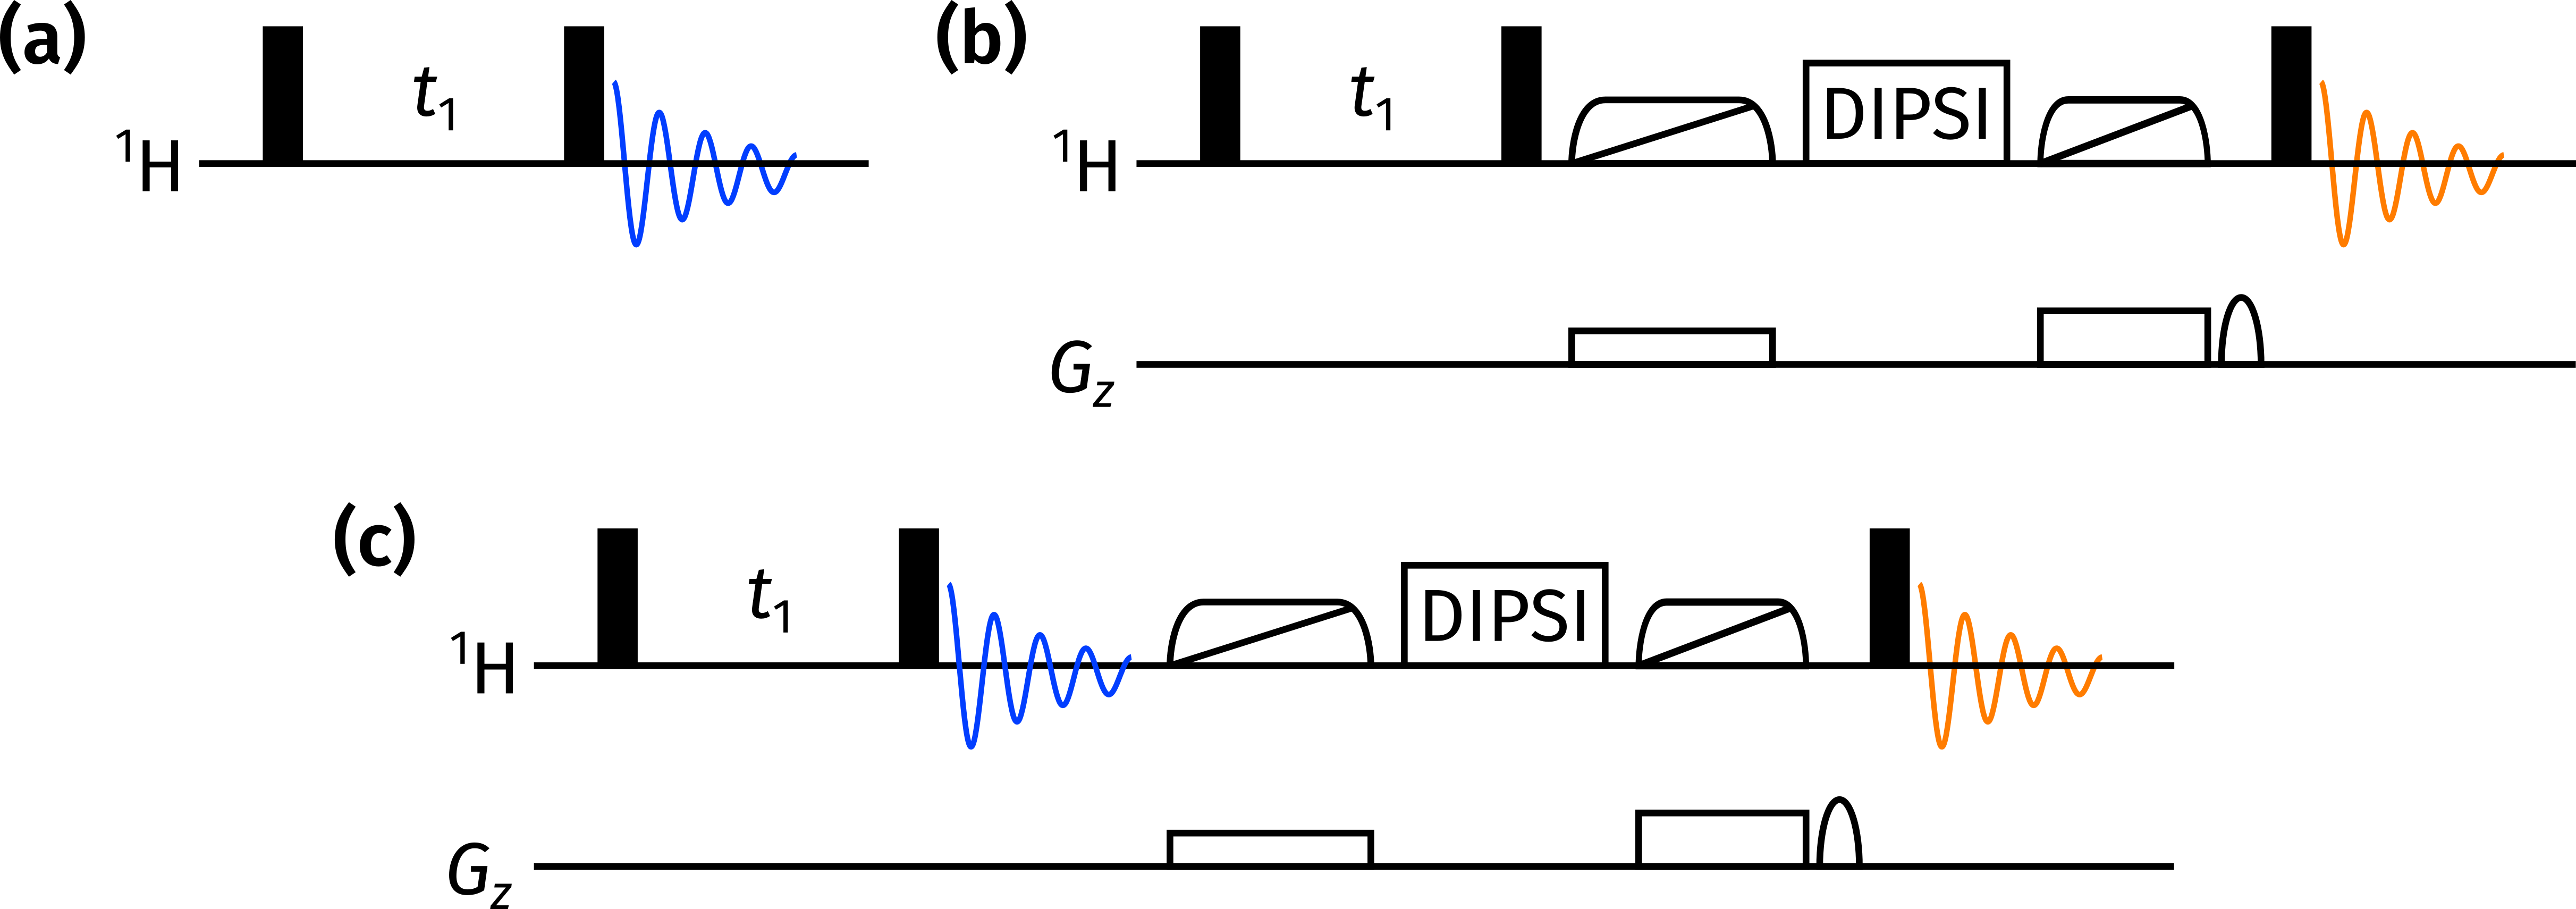
\includegraphics[]{pp/ct_states.png}%
    {\phantomsubcaption\label{fig:ct_states_c}}%
    {\phantomsubcaption\label{fig:ct_states_t}}%
    {\phantomsubcaption\label{fig:ct_states_ct}}%
    \caption[COSY/TOCSY NOAH module]{
        \textbf{(\subref{fig:ct_states_c})} COSY module.
        \textbf{(\subref{fig:ct_states_t})} TOCSY module; zero-quantum suppression is employed before and after the isotropic mixing period.
        \textbf{(\subref{fig:ct_states_ct})} Combined COSY/TOCSY module, where the COSY FID is acquired immediately before the TOCSY mixing.
    }
    \label{fig:ct_states}
\end{figure}

As shown in \cref{tbl:noah_sensitivities} (entry 2), this nesting of the COSY module does not materially affect the TOCSY sensitivity.
A small loss of approximately 20\% is observed, which is partly due to the imperfect magnetisation preservation by the HSQC, and perhaps also due to relaxation during the COSY acquisition period.
As for the time-saving factor, a slightly larger deviation ($\rho_t = 2.60$) is observed from the ideal value of $3$.
This reflects the addition of a TOCSY mixing period, which contributes to $\tau_\text{ps}$.

\subsubsection{\noah{B,S}: HMBC + HSQC}

As mentioned previously, the HMBC module shown in \cref{fig:noah_sb_po_b} is designed to retain \magn{C} magnetisation through the addition of the $zz$-filter.
This can be used in a subsequent HSQC module in a \noah{B,S} supersequence.
Entry 3 of \cref{tbl:noah_sensitivities} shows that the addition of the $zz$-filter to the HMBC causes a relatively small 7\% decrease in sensitivity; on the other hand, the HSQC loses 13\% of its sensitivity because of incomplete magnetisation preservation.

Generally, it has been recommended that less sensitive modules are placed earlier in the supersequence so that they can access a larger proportion of the equilibrium magnetisation.
Since the HMBC is less sensitive of the two modules, this rule of thumb suggests that the BS supersequence would be better than the alternative SB supersequence.
In fact, the opposite is true, as entry 4 of \cref{tbl:noah_sensitivities} shows.
The HSQC module has a boost in sensitivity because it is placed first in the supersequence, and no longer needs to rely on the \magn{C} magnetisation preserved by the HMBC; and the HMBC also benefits because the $zz$-filter modification is no longer needed.%
\footnote{In fact, the final \ang{180} pulse in the HMBC module could also be removed: this is likely to give a further boost in SNR, as discussed in \cref{subsec:noah__hmbc}. However, this was not done here.}
Arguably, the ordering of modules in a supersequence should be considered on a case-by-case basis.

\subsubsection{\noah{B,S,C,T}: HMBC + HSQC + COSY + TOCSY}

We now move on to a longer supersequence containing four modules, with a correspondingly larger $\rho_t$ value of 3.22.
The sensitivity of the HSQC module is practically the same as in the \noah{B,S} supersequence just described: however, the COSY and TOCSY modules expose one weakness of the HMBC module which has so far been overlooked.
In principle, the HMBC module should only excite magnetisation of protons which are long-range coupled to \carbon{} (which we could, for example, denote as \magn{C(LR)}).
This magnetisation pool should be separate from both the directly coupled protons (\magn{C}), as well as protons which are not coupled to any \carbon{} at all (\magnnot{C}).
Unfortunately, this is not the case: it is not actually possible to separate the \magn{C(LR)} and \magnnot{C} magnetisation pools.
The HMBC excites both of these magnetisation sources, dephases the latter using CTP gradients, and detects the signal arising from the former.

What this means, of course, is that the COSY/TOCSY module which rely on \magnnot{C} magnetisation will have substantially lower sensitivities.
The signal detected in these two modules derives only from whatever has recovered during the previous two acquisition periods, as shown in entry 5 of \cref{tbl:noah_sensitivities}: $A$ for COSY and TOCSY is 0.36 and 0.28 respectively.
That said, this is in fact not likely to be an issue \textit{even} for sensitivity-limited samples.
Because the intrinsic sensitivity of the HMBC is orders of magnitude lower than the COSY and TOCSY, even with these large losses in sensitivity, the COSY and TOCSY spectra still have greater intensities than the HMBC.
Thus, as long as the entire supersequence is acquired with enough scans to make the HMBC SNR sufficient, the SNR in the COSY and TOCSY will \textit{also} be acceptable.
This is illustrated in \cref{fig:bsct}.

A rather more insidious problem is that different signals relax at different rates: thus, the COSY and TOCSY spectra (or indeed, any homonuclear module) will have uneven intensities and are frequently asymmetric.
This can be seen in the COSY spectrum, where a pair of asymmetric crosspeaks are highlighted.
Adding a period of isotropic mixing before the COSY module\autocite{Kupce2018CC} can help to ameliorate this to some extent (this was not performed when acquiring the data in \cref{fig:bsct}).

\begin{figure}[!ht]
    \centering
    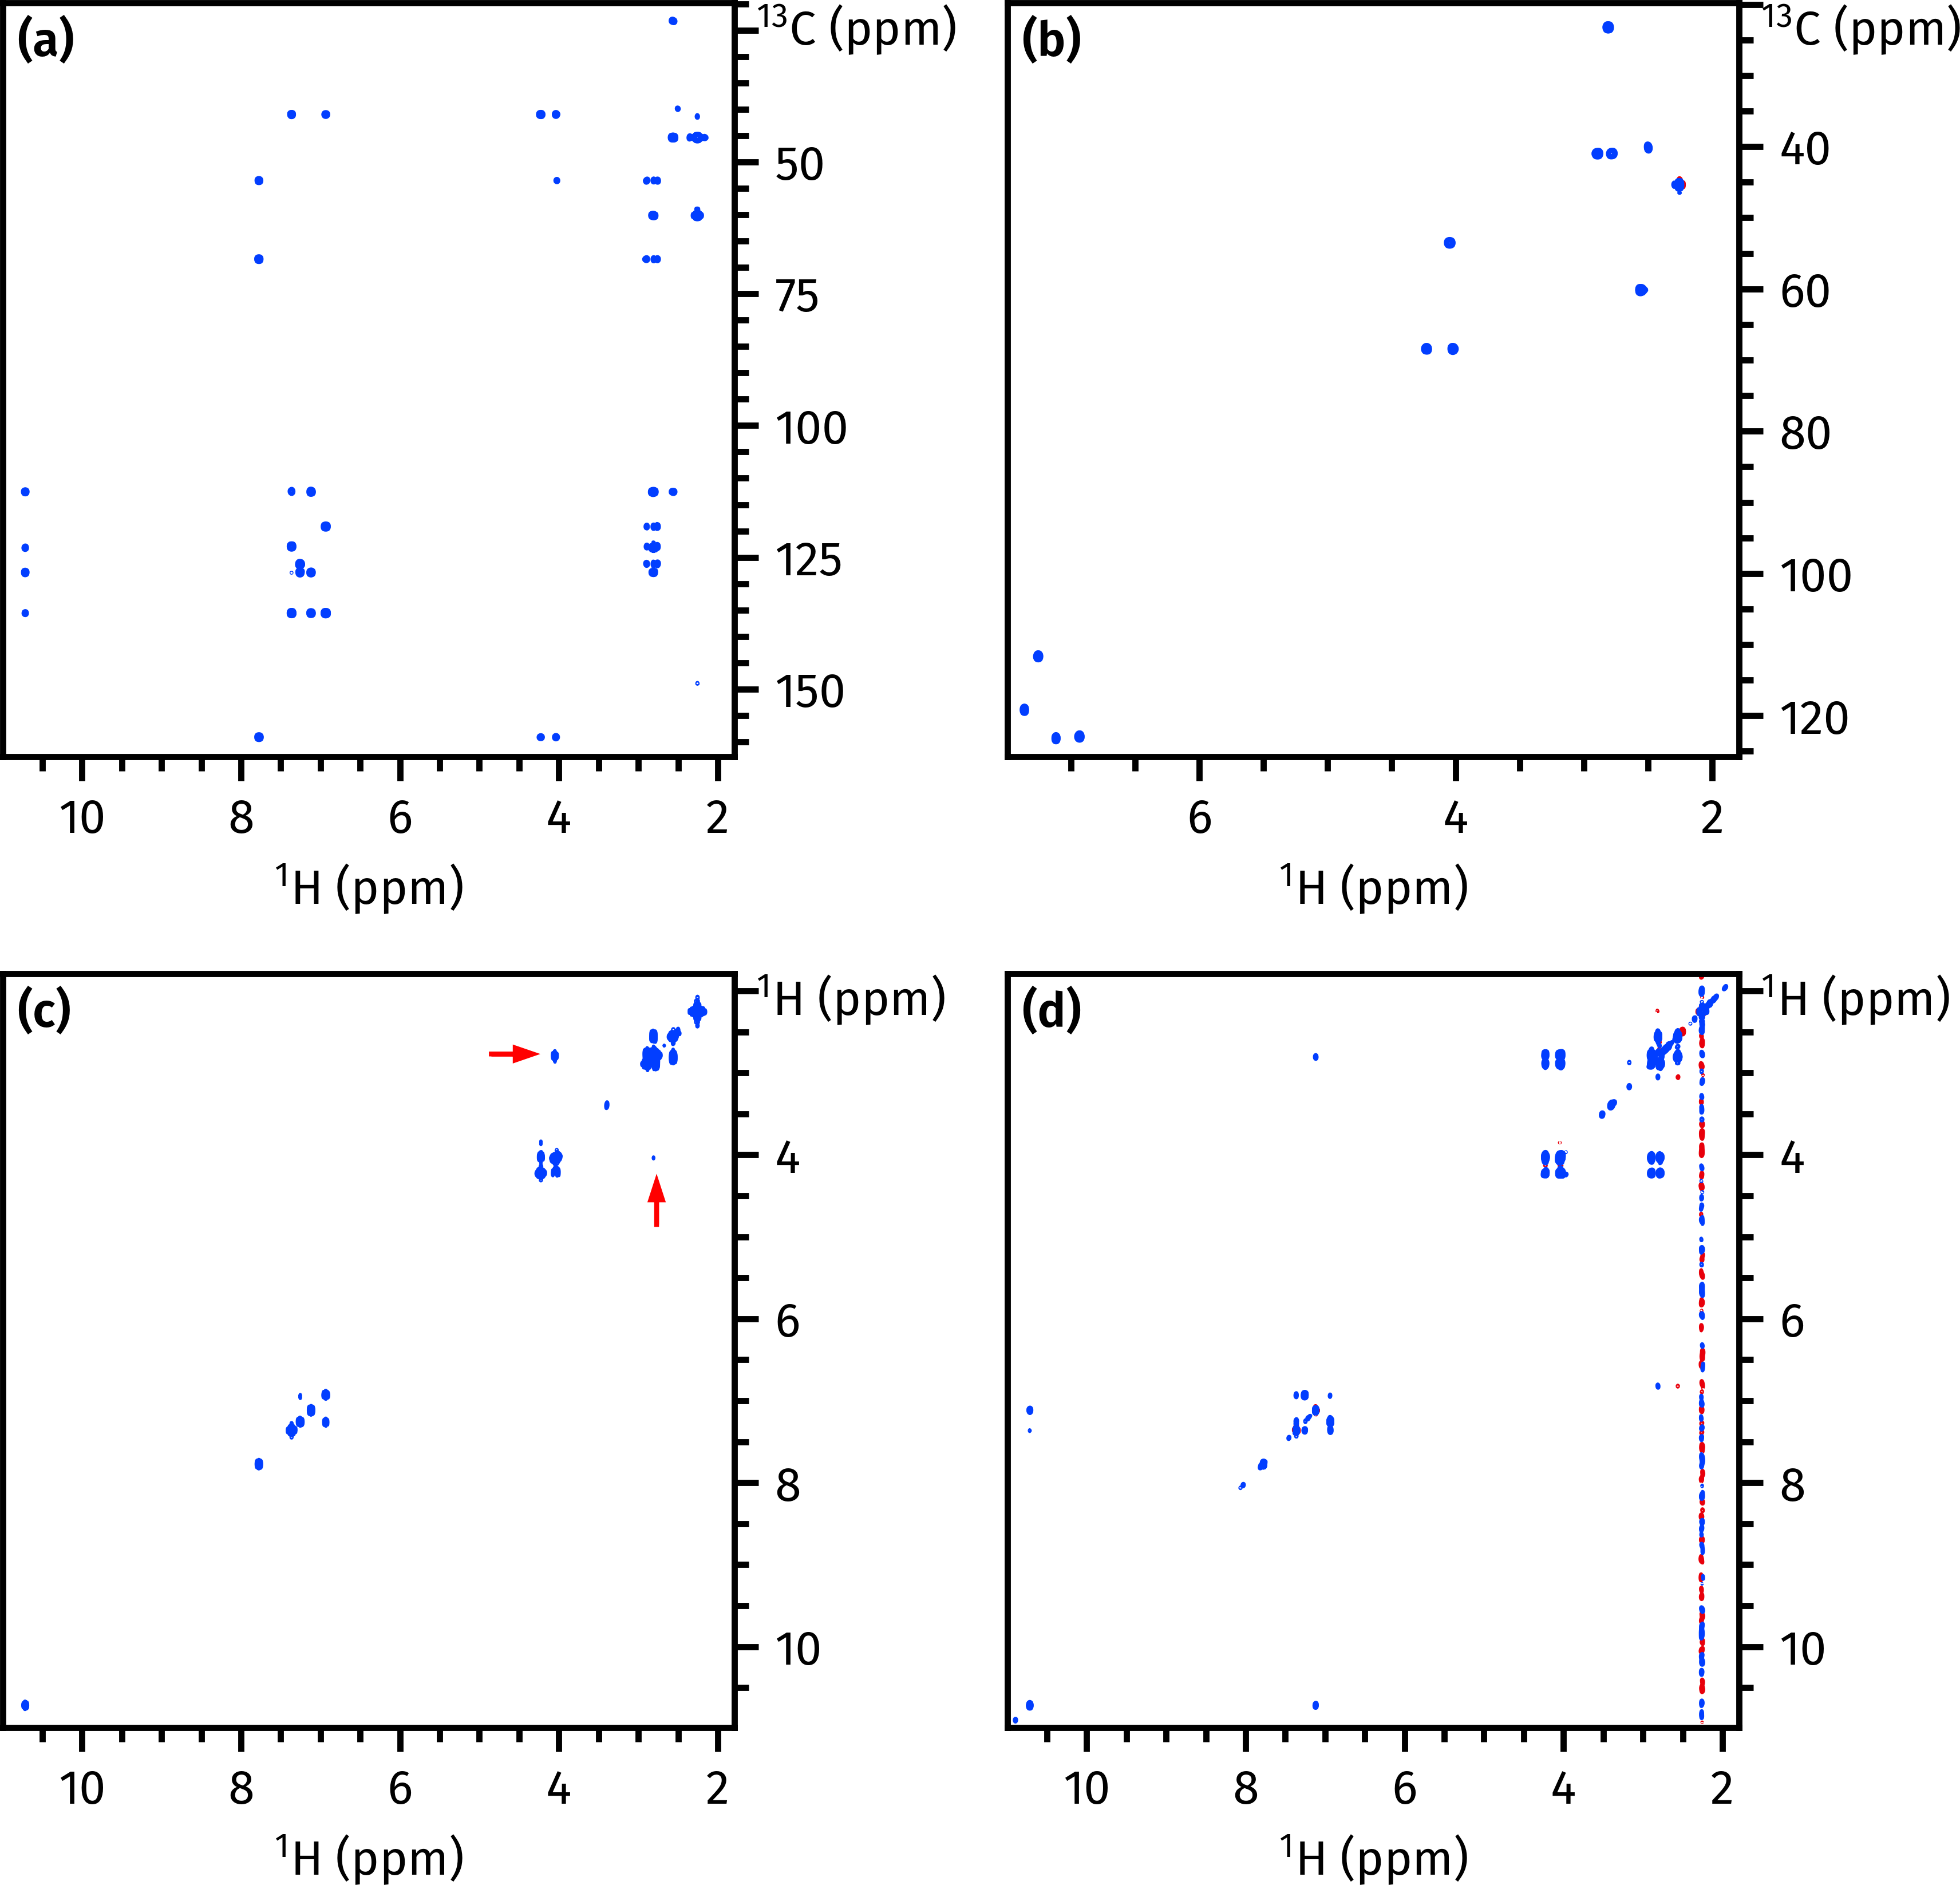
\includegraphics[]{noah/bsct.png}%
    {\phantomsubcaption\label{fig:bsct_b}}%
    {\phantomsubcaption\label{fig:bsct_s}}%
    {\phantomsubcaption\label{fig:bsct_c}}%
    {\phantomsubcaption\label{fig:bsct_t}}%
    \caption[Spectra obtained from a \noah{B,S,C,T} supersequence.]{
        Spectra obtained from a \noah{B,S,C,T} supersequence. 
        \textbf{(\subref{fig:bsct_b})} HMBC.
        \textbf{(\subref{fig:bsct_s})} HSQC.
        \textbf{(\subref{fig:bsct_c})} COSY; a pair of asymmetric crosspeaks are highlighted with red arrows.
        \textbf{(\subref{fig:bsct_t})} TOCSY (\qty{60}{\ms} DIPSI-2 mixing).
        Despite the COSY and TOCSY having only $\sim$ 30\% sensitivity compared to standalone experiments, the intensity of the spectra obtained is still perfectly acceptable (the contour levels chosen are 1--2 orders of magnitude larger than for the HMBC).
        \datacode{7Z-220224}
    }
    \label{fig:bsct}
\end{figure}


\subsubsection{\noah{B,Spn,S,C,T}: HMBC + \nitrogen{} seHSQC + HSQC + COSY + TOCSY}

As the final example, we add a further magnetisation pool to the mix, namely protons directly coupled to \nitrogen{} (i.e.\ \magn{N}).
As of the time of writing, the implementation of multiple-FID experiments on Bruker spectrometers limits $N$ to a maximum of 5, so a supersequence such as the present \noah{B,Spn,S,C,T} is the current limit.
(However, there is no \textit{scientific} argument forbidding $N > 5$, and it is likely that in future versions of TopSpin this restriction will be lifted.)

The values of $A$ for each module are given in entry 6 of \cref{tbl:noah_sensitivities}.
If the HMBC module is placed at the beginning of the supersequence, then in order to preserve \textit{both} \magn{N} and \magn{C} magnetisation, the $zz$-filter must be extended to include \nitrogen{} pulses\autocite{Kupce2019JMR}.
As before, the \nitrogen{} seHSQC and \carbon{} HSQC modules both suffer drops in sensitivity.
For the \nitrogen{} seHSQC, this is partly because of imperfect preservation of \magn{N} magnetisation by the HMBC, but also stems from the addition of the $zz$ isotope-selective pulse (ZIP) element to the seHSQC pulse sequence; this is described further in \cref{subsec:noah__sehsqc_n}.
On the other hand, for the \carbon{} HSQC, the sensitivity loss stems purely from imperfect retention of \magn{C} magnetisation.
Finally, because the HMBC dephases \magn{!X} magnetisation, the COSY and TOCSY at the end have lower sensitivities: however, as discussed above, this is not an issue in practice.

It is also possible to move the \nitrogen{} seHSQC module to the front: this gives it a slightly greater sensitivity, at the cost of the HMBC (entry 7, \cref{tbl:noah_sensitivities}).
In general, these two modules tend to have comparable sensitivity, and which of these two arrangements is better depends on which module the sensitivity needs to be optimised for.

Lastly, the value of $\rho_t$ given here of 3.74 represents an effective upper limit on the time-saving factor.
Although $\rho_t$ increases with $N$, the extent to which it deviates from the ideal value of $N$ also increases: it is very difficult to obtain $\rho_t > 4$, even with five modules in the supersequence.
Of course, it is possible to increase $\rho_t$ further by lengthening the recovery delay $d_1$ used for the experiments: for example, if $d_1$ is increased to \qty{2}{\s} from its present value of \qty{1.5}{\s}, $\rho_t$ increases to 3.94.
Obviously, this can only be pushed so far before it becomes meaningless.
